\documentclass{book}
\usepackage{pdfpages} %paquete que permite agregar pdfs

\begin{document}

    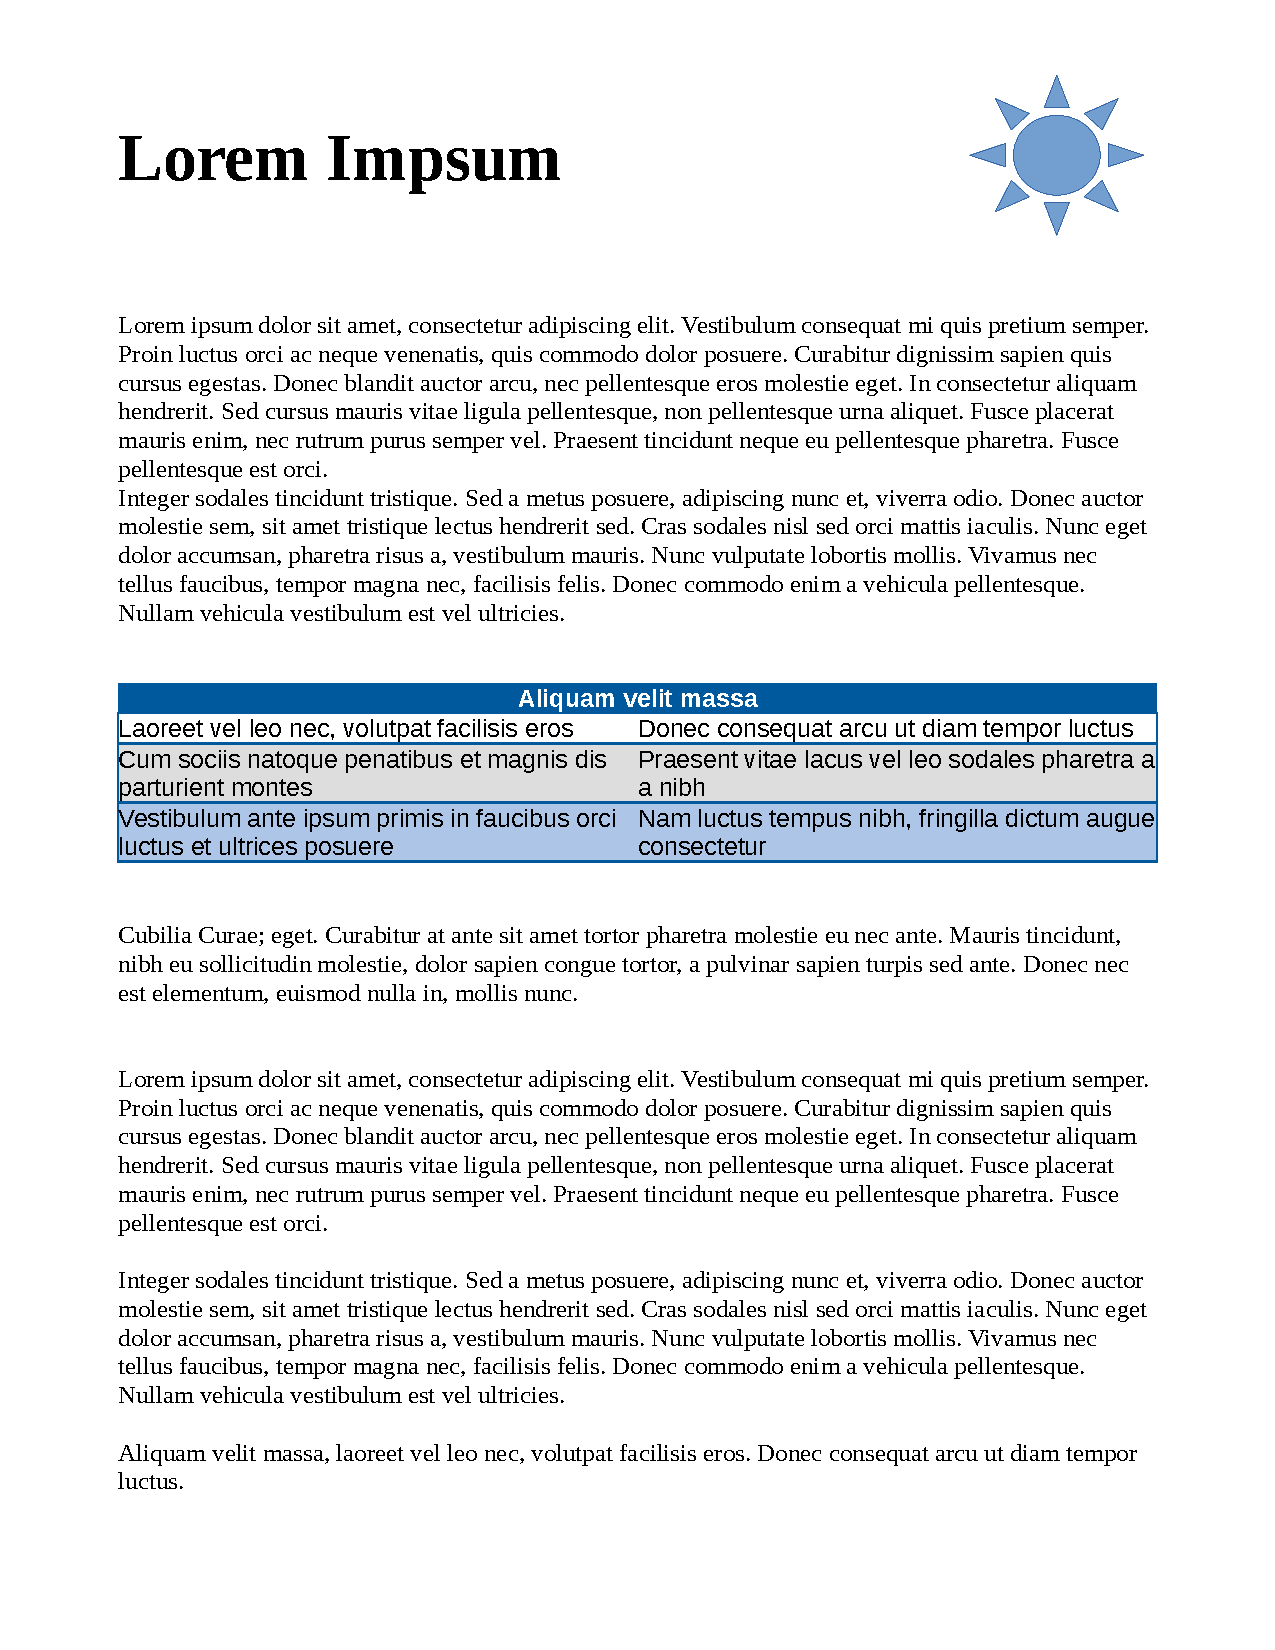
\includepdf[pages=-,fitpaper=true]{documento1.pdf}
    
\includepdf[pages=-,fitpaper=true]{documento2.pdf}
    %\includepdf[pages=-,fitpaper=true]{documento3.pdf}

    %%%%%%%%%%%
    % pages=-       significa que se van a agregar todas las paginas del archivo pdf
    % fitpaper=true significa que el documento se va a incluir con sus medidas de hoja originales
    % se pueden agregar mas pdfs al archivo agregando mas lineas de tipo \includepdf[pages=-,fitpaper=true]{archivo.pdf}
    %%%%%%%%%%%

\end{document}